
%\documentclass[a4paper,twocolumn, 10pt]{article}
\documentclass[conference]{IEEEtran}


%%% 그림 관련
\usepackage[dvips]{graphicx}
\usepackage{subfigure}

\begin{document}

\title{Abnormal Object Detection Using Second-Order Spatio-Temporal Background Model}
\author{Suil Son, Young-Woon Cha, and Suk I. Yoo}

\maketitle

\begin{abstract}
This paper presents the robust background subtraction method in dynamic background constraints.

One problem of other methods is that as they used color-based density estimation, they could suffer from the so-called camouflage problem. This typically occurs when the color is similar to its background even when its shape is sharply different. Thus, shape features should be combined to the background model.

Moreover, since dynamic backgrounds are varying frequently, other first-order background subtraction methods gives unwanted false-alarms in those images due to the variance of the background. Thus, the background model should be extended to include nonstaionary background as normal.

This paper suggests the spatio-temporal background model by introducing shape features and demonstrates significant improvements in detection. This paper also proposes the variation subtraction method by extending background model into the second-order space. After variation subtraction, the stable response on dynamic background images facilitates reliable thresholding for abnormality decision.

The proposed method was tested on Natural scenes with dynamic background for object recognition and Semi-conductor wafer SEM (Scanning electron microscope) images with noise for defect detection. Experiments show that our algorithm enhanced the discrimination and successfully suppressed false-alarms from dynamic background.

\textbf{Keywords}: background subtraction, defect detection, foreground detection, object recognition, shape matching

\end{abstract}

\IEEEpeerreviewmaketitle


\section{Introduction}
The main goal of the visual surveillance in computer vision is to classify abnormal events based on prior or domain knowledge. The prior knowledge can be expressed by modeling normality using training examples. If given inspection data is similar to the training examples, they are classified as background (normal pattern) and others as foreground (abnormal pattern). This problem is called Foreground detection.

  The background subtraction methods have been proposed to deal with the problem. The stationary background assumption of those methods is that images are captured by fixed camera, and that those images consist of stationary background. The stationary background has the consistency with respect to color and its position. Those approaches can be applied to various areas such as object recognition, object tracking, defect detection, and visual surveillance.

  However, the development of robust background model has been demanding to contain dynamic backgrounds. The stationary background assumption is violated if their images contain dynamic backgrounds. That is, the conventional background model could not sufficiently explain followings: the camouflage foreground which color is similar to its background and the dynamic background which position has been frequently changed.
 
  Dynamic background constraints are natural conditions in object recognition and defect detection. The dynamic images appear where natural scenes with nonstationary objects such as swaying trees, fountains, moving cars and people. Dynamic background images also include misalignment images captured by hand-held cameras and include noised images – highly zoomed-in images, and dynamic textured images. Semi-conductor wafer SEM (Scanning electron microscope) images are one example. Even after alignments of those dynamic background images, small misalignments remain due to the variance of the background. Other methods mostly conducted their experiments on video, but the suggested method regards the input as a set of independent images with respect to time for applying to general applications. 
      
Some problems, however, occur when using the first-order color-based background subtraction methods to deal with the dynamic background images. The color-based background models could suffer from the so-called camouflage problem. (See figure \ref{fig:10}). False-negatives occur when its color is similar to its background even when their shapes are sharply different. Thus, shape features should be combined into the background model. 

\begin{figure}[!t]
  \centering
  \label{fig:10}
  \subfigure[ ]{
\includegraphics[width=0.15\textwidth]{paper-fig/fig10-1}}\hfill
  \subfigure[ ]{
\includegraphics[width=0.15\textwidth]{paper-fig/fig10-2}}\hfill
  \subfigure[ ]{
\includegraphics[width=0.15\textwidth]{paper-fig/fig10-3}}
  \caption{Camouflage Problem. The third column shows the foreground detection result using stationary background model. The camouflage foregrounds were misclassified though their shapes are sharply different to the background}
\end{figure}

\begin{figure}[!t]
  \centering
  \label{fig:20}
%  \subfigure[ ]{\includegraphics[width=0.15\textwidth]{paper-fig/fig20-1}}\hfill
  \subfigure[ ]{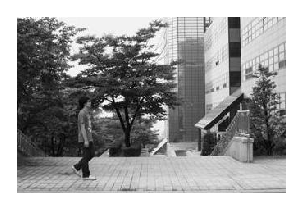
\includegraphics[width=0.23\textwidth]{paper-fig/fig20-2}}\hfill
  \subfigure[ ]{
\includegraphics[width=0.23\textwidth]{paper-fig/fig20-3}}
  \caption{Imbalance of background density. The first row illustrates a dynamic background image. There are swaying trees and small misalignments. The second row shows intensity distribution of the background in three different regions and straight lines are global thresholds. The third row represents detection result. Note that since other background subtraction methods try to classify foregrounds using a single threshold, false-positives are increased due to the imbalance among each background density.}
\end{figure}


Moreover, as dynamic backgrounds are varying frequently, the stationary background model based approaches generate many false-positives in those images due to the imbalance among each background density. (See figure \ref{fig:20}). Thus, the background model should be extended to include nonstaionary backgrounds as normal. 
This paper presents the robust background model for containing dynamic backgrounds. In Section 2, the previous works and background works for the proposed method are discussed. 

The proposed work has two novel contributions: Firstly, the background is modeled on the shape-intensity joint domain, so it can estimate shape and intensity change simultaneously and improves discrimination compared to other intensity-based background models. Secondly, since background dynamics can be explained in the second-order space, we suggest the second-order background model for removing background’s variation. The suggested variation subtraction method generates stable response on dynamic background images and thus the threshold selection methods can be reliably applied to this model. In Section 3, 4, the suggested formulation and detailed algorithm is presented.

This method was tested on Natural scenes with dynamic background for object recognition and Semi-conductor wafer SEM images with noise for defect detection. The results show that the algorithm enhanced discrimination and successfully suppressed false-alarms from dynamic background. In Section 5, 6, detailed analysis and the experimental results are discussed, respectively.



\section{Related Work}

Background subtraction approaches can be categorized by their feature space. The first background subtraction methods \cite{Piccardi, Wren, Cucchiara} suggested statistical methods based on temporal consistency by assuming the single background modal. Single Gaussian \cite{Wren} or median \cite{Chucchiara} was used for modeling background. Then, the mixture of Gaussians \cite{Stauffer} was introduced for extending background model to the multi-modal. 

Non-parametric background model using kernel density estimation \cite{Elgammal} was introduced. The rest of the background subtraction algorithms also have used kernel density estimation for measuring similarity between inspection data and training data. To find the probability that a point \begin{math} x \end{math}  belongs to training example \begin{math} \hat{x} \end{math} , an estimate can be computed as,
\begin{equation}\label{eq:10}
  P_N( \mathbf{x} ) = \frac{1}{n} \sum_{j=1}^N \frac{1}{h^D}K \Big( \frac{ \mathbf{x} - \hat{\mathbf{x}}_j } {h} \Big)
\end{equation}
where \begin{math} h \end{math} is a symmetric positive definite \begin{math} D \times D \end{math} bandwidth matrix. ` \begin{math} \hat{} \end{math} ' denotes training example. The d-variate Gaussian function is a common choice as the kernel function \begin{math} K \end{math}, 
\begin{equation}\label{eq:20}
  p( \mathbf{x} ) = \frac{1}{N} \sum_{j=1}^N (2\pi)^{-D/2} |\mathbf{H}|^{-1/2}
                    exp \Big( -\frac{1}{2} (\mathbf{x} - \hat{\mathbf{x}}_j)^T |\mathbf{H}|^{-1}  (\mathbf{x} - \hat{\mathbf{x}}_j ) \Big) 
\end{equation}

The kernel function has a role in transforming the distance of \begin{math} (x , \hat{x}_j) \end{math}  into the probability of their similarity. Then, the average probability of similarity is taken. The bandwidth \begin{math} h \end{math} represents a generalization preference for decision. Data-driven bandwidth selection methods have been proposed, \cite{Jones, Comaniciu}.

Proximal neighborhoods' smoothness assumption was considered for robustness of the likelihood. \cite{Elgammal} used joint distribution among proximal neighborhoods. \cite{Sheikh} tried discontinuity preserving smoothing for false-alarm suppression using graph-cut assuming the morphological smoothness.

Another attempt for robustness is that \cite{Sheikh} suggested the likelihood ratio test between the background likelihood and the uniform distribution, so the likelihood values can be more stretched. \cite{Ko} regarded proximal neighbors \begin{math} x^C \end{math} of \begin{math} x \end{math} as single component and compared the component's intensity histogram. The method showed the component consistency is more important than single pixel consistency. \cite{Mittal} estimated background density via variable bandwidth kernels for better data-driven estimation.

The attempts to deal with positional distribution were also introduced assuming that pixel positions can be changed in dynamic background. \cite{Elgammal} corrected small misalignments by searching best correspondents in near positions. \cite{Sheikh} incorporated position variable with temporal variable jointly. It searched best correspondence on entire positions for handling dynamic positional change.

\cite{Mittal} tried to combine another features into background model such as normalized color, and motion. They introduced motion information as a spatial relation parameter using optical flow assuming that intensity and optical flow features are uncorrelated. The result showed motion information is important for recognition. Consequently, the work implies that background density should be estimated based on both spatial and temporal domain.

  Background Variation Modeling approaches \cite{Jodoin, Bebezeth} have been proposed. The background’s behavior was captured by given labeled motion images. Labeled motion images \begin{math} L(x) \in \{0, 1\} \end{math}  are binary and acquired after simple background subtraction. Their main assumption is that the change of the binary motion label explains background's behavior. Therefore, \cite{Jodoin, Bebezeth} estimate the background variation by taking expectation of the classification rate from given labeled images. In the inspection stage, two subtractions are performed. The former is the simple background subtraction and the latter is the variation subtraction. Due to the second stage, varying backgrounds are classified to normal 

Shape matching algorithms define a shape as a gradient distribution with respect to space. The direct use of gradients is quite sensitive, so derivative of Gaussian (DoG) can be used in order to reduce noise effect, [13].
\begin{equation}\label{eq:30}
  \frac{d}{dx}(G*I) = \Big( \frac{d}{dx}G \Big) * I
\end{equation}
\begin{equation}\label{eq:40}
  G^{\prime}(x) = - \frac{x}{ \sigma ^2} e^{ - \frac{x^2}{2\sigma ^2}}
\end{equation}
After separable convolution, \begin{math} G_x \end{math} and \begin{math} G_y \end{math} are obtained. \cite{Mikolajczyk, Belongie} commonly used log-polar coordinates for robust spatial representation. By transforming the \begin{math} (x, y) \end{math} gradients in Cartesian coordinates into \begin{math} (\theta, d) \end{math} polar coordinates, a shape of each point is determined by two parameters, angle and distance respectively. Changing polar coordinates can be computed as,
\begin{equation}\label{eq:50}
  \theta = \textrm{tan}^{-1} \Big( \frac{I_y}{I_x} \Big)
\end{equation}
\begin{equation}\label{eq:60}
  |\nabla I| = \sqrt{I_x^2 + I_y^2 }
\end{equation}

The feature vector of the log-polar coordinates is defined as \begin{math} X \equiv ( \theta, log(|\nabla I|) ) \end{math}. The angle parameter \begin{math} \theta \end{math} indicates a shape of a point. The distance parameter \begin{math} log(|\nabla I|) \end{math} captures a degree of flatness or edgeness. The log-scaled distance is used for reducing sensitiveness. Figure \ref{fig:30} represents Cartesian coordinates and log-polar coordinates. Note that flat regions only have small distances but they could have divergent angles among them due to the noise. In this case, the \begin{math} \theta \end{math} is meaningless, so it is desirable to set to \begin{math} \theta = 0 \end{math}, if \begin{math} log(|\nabla I|) < 1 \end{math}. 

\begin{figure}[!t]
  \centering
  \label{fig:30}
%  \subfigure[ ]{\includegraphics[width=0.15\textwidth]{paper-fig/fig30-1}}\hfill
%  \subfigure[ ]{\includegraphics[width=0.15\textwidth]{paper-fig/fig30-2}}
  \caption{Log-polar Representation}
\end{figure}

Shape matching algorithms find similar shapes by comparing spatial distribution among two local histograms. For measuring the spatial similarity, \begin{math} \chi ^2 \end{math} test is commonly used, \cite{Belongie}:
\begin{equation}\label{eq:70}
  C_{ij} \equiv C( p_i, q_j ) = \frac{1}{2} \sum_{k=1}^K 
                              \frac{[h_i(k) - h_j(k) ] ^2}{h_i(k) + h_j(k) }
\end{equation}
\begin{math} h_i(k) \end{math} and \begin{math} h_j(k) \end{math}  denote the \begin{math} K \end{math}-bin normalized histogram at \begin{math} p_i \end{math} and \begin{math} p_j \end{math}, respectively. (7) is equivalent to the likelihood ratio test in \cite{Sheikh, Bebezeth}.


\section{Spatio-Temporal Consistency}
The suggested method considers spatial and temporal consistency jointly to estimate how much given inspection image is consistent with training examples. The spatial relation can be expressed by Shape distribution with respect to space. Also, the temporal relation can be represented by intensity distribution over time. Thus, the problem domain can be modeled in the structure of Spatio-Temporal Markov Random Field Model \cite{Kamijo}. The proposed method is formulated based on the S-T MRF model.

Figure \ref{fig:40} shows the relation of Spatio-Temporal neighborhood on training image set. Each parallelogram represents a training image. A point \begin{math} \hat{x}_n^{i,j} \end{math}  denotes \begin{math} (i, j) \end{math} pixel on nth training image having \begin{math} x \end{math} intensity. Subscript indicates temporal neighborhoods of \begin{math} x \end{math}. Temporal consistency means that an intensity of a point \begin{math} x \end{math} on inspection image should be statistically consistent with the intensities of \begin{math} \hat{X} \equiv ( \hat{x}_1, ..., \hat{x}_N)^T \end{math}. 

Also, \begin{math} \hat{x}_i^C \end{math} represents spatial neighborhoods of \begin{math} \hat{x}_i \end{math}, such that \begin{math} \hat{x}^C = \{ x^{a,b} | |a-i| < c, | b - j | < c \} \end{math} . Thus, the spatio-temporal consistency means that a component  \begin{math} \hat{x}^C \end{math}  should be statistically consistent with  \begin{math} \hat{X} \equiv [( \hat{x}_1^C), ..., (\hat{x}_N^C) ]^T \end{math}. To avoid the curse of dimensionality, the spatial relation of \begin{math} x^C \end{math} can be parameterized using gradients. Thus, \begin{math} P(Spatial,Temporal) \end{math} is equivalent to \begin{math} P(component) \end{math}. The spatio-temporal consistency can be represented by \begin{math} P(Shape, Intensity) \end{math}. 

\begin{figure}[!t]
  \centering
  \label{fig:40}
  \subfigure[ ]{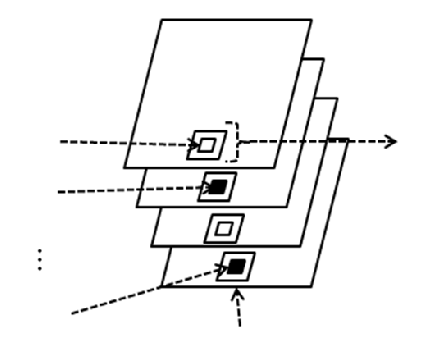
\includegraphics[width=0.23\textwidth]{paper-fig/fig40-1}}\hfill
  \subfigure[ ]{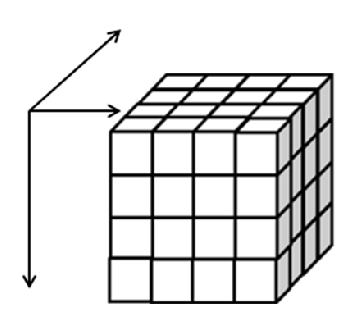
\includegraphics[width=0.23\textwidth]{paper-fig/fig40-2}}
  \caption{Spatio-Temporal Neighborhood}
\end{figure}


\subsection{Suggested Formulation}
The suggested approach estimates both background's density and its variation for dynamic background subtraction. The main procedure has two stages. (See \ref{fig:40}. In the training stage, a set of foreground likelihood \begin{math} \hat{L}_i \end{math} is estimated from given a set of positive images \begin{math} \hat{I}^+ \end{math}  using first-order background subtraction based on \begin{math} P(Shape, Intensity) \end{math} . Then, the background variation model is assumed to be a uni-modal for speed and compact representation. It can be estimated simply by taking expectation of \begin{math} \hat{L}_i \end{math} . In the inspection stage, first-order background subtraction and second-order variation subtraction are linearly performed. By matching similarity between a foreground likelihood \begin{math} E(\hat{L}) \end{math}  and an expected likelihood \begin{math} \hat{L}^2 \end{math} , a second-order foreground likelihood   can be estimated.

\begin{figure}[!t]
  \centering
  \label{fig:50}
  \subfigure[ ]{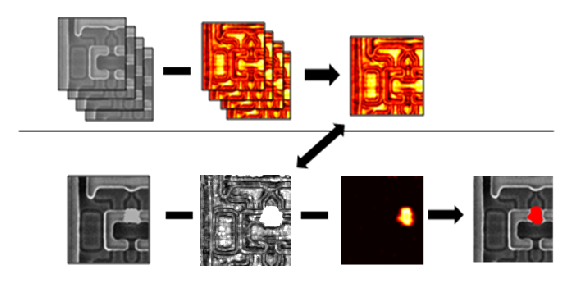
\includegraphics[width=0.5\textwidth]{paper-fig/fig50}}
  \caption{Spatio-Temporal Neighborhood}
\end{figure}


\section{Spatio-Temporal Consistency}

\subsection{First-order Spatio-Temporal Background Model}
In order to estimating \begin{math} P(spatial, temporal) \end{math} , the feature space is defined on the S-T MRF as,
\begin{equation}\label{eq:80}
  \mathbf{x} \equiv (\theta, log(|\nabla I|), I)
\end{equation}
The first two variables are for a spatial relation that is represented by log-polar representation using (\ref{eq:40}), (\ref{eq:50}), (\ref{eq:60}), The third variable represents a temporal relation using intensity. Therefore, the S-T background model for each pixel x describes joint distribution of temporal and instant spatial relation. 

A probability of normality \begin{math} P_N(\mathbf{x} \end{math}  on S-T domain can be estimated using (\ref{eq:10}) (\ref{eq:80}). Figure \ref{fig:60} shows examples of S-T background density. Note that the dynamic regions are containing multi-modal density, while static regions are maintaining uni-modal density.

\begin{figure}[!t]
  \centering
  \label{fig:60}
  \subfigure[ ]{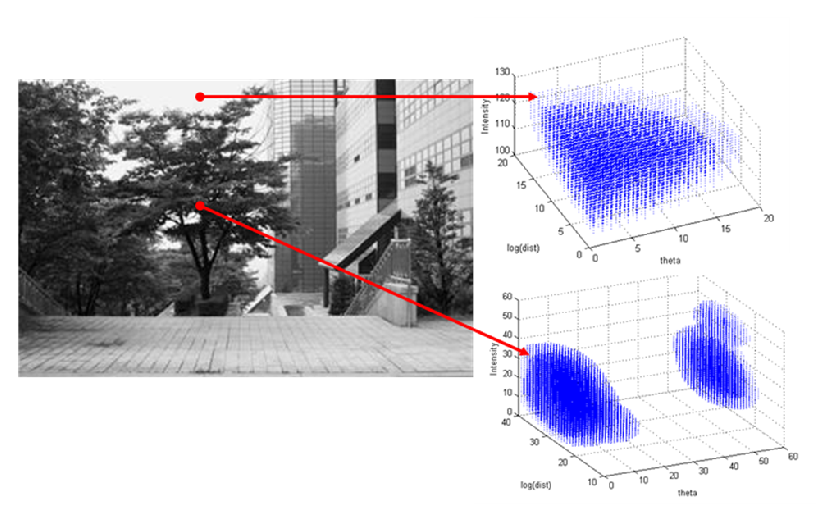
\includegraphics[width=0.5\textwidth]{paper-fig/fig60}}
  \caption{Spatio-Temporal Background Distribution}
\end{figure}

\begin{equation}\label{eq:90}
  P(x^c) \propto \prod_{k \in x^C} \psi ^k (k)
\end{equation}
In MRF, a joint distribution \begin{math} P(x^C) \end{math}  is proportional to a product of potential functions \begin{math} \psi^k(k) \end{math}  over the maximal cliques \begin{math} P_N(\mathbf{x} \end{math} , \cite{Bishop}. Thus, a component probability \begin{math} P_N(\mathbf{x}^C \end{math}  can be calculated using \begin{math} P_N(\mathbf{x} \end{math}  and is containing broader spatio-temporal relation. Also, the log of the likelihood ratio test \cite{Sheikh} is used as a potential function \begin{math} \psi^k(k) \end{math} . Therefore, the first-order foreground likelihood \begin{math} \tilde{L}_x(x) \end{math} can be calculated as,
\begin{equation}\label{eq:100}
  \tilde{L}_x(x) = \frac{1}{C} \sum_{i=1}^C - \textrm{ln} \frac{P_N(x)} {P_A(x)}
\end{equation}
\begin{equation}\label{eq:110}
  P_A(x) = \frac{1}{| \theta | \cdot |logr| \cdot |i|}
\end{equation}
The probability of abnormality \begin{math} P_A(x) \end{math} is assumed as a uniform distribution. The \begin{math} C \end{math} is the number of neighborhood. In experiments, 3 \begin{math} \times \end{math} 3 patch is used as a component \begin{math} x^C \end{math}. 
%%%
\begin{equation}\label{eq:120}
  \tilde{L}(x) = \textrm{min}_{y \in x^C}  (\tilde{L}_y(x))
\end{equation}
%%%
In addition, positional distribution is considered using (\ref{eq120}) for handling small displacement on dynamic background. In experiment, displacement within one pixel was corrected by finding best correspondence in near eight-neighbors. \begin{math} y \end{math} is the neighborhood of \begin{math} x \end{math}. \begin{math} \tilde{L}_y(x) \end{math}  is calculated at \begin{math} y \end{math} position using the feature values of \begin{math} x \end{math}.


\subsection{Second-order Spatio-Temporal Background Model}
Background variation can be captured by \begin{math} \tilde{L}_y(\hat{x}) \end{math}  distribution and the Expected likelihood descriptor \begin{math} E(L) \end{math} can be built for containing the variation. By assuming temporally and spatially uni-modal, \begin{math} E(L) \end{math} becomes a virtual reference image. It is computed by taking expectation of \begin{math} \tilde{L}_y(\hat{x}) \end{math} with respect to time. 
\begin{equation}\label{eq:130}
  E(\tilde{L}_y(\hat{x})) = \frac{1}{N} \sum_{j=1}^N \tilde{L}_y(\hat{x}_j)
\end{equation}
where \begin{math} N \end{math} is the number of \begin{math} \hat{I}^+ \end{math} . Figure \ref{fig:70} shows an example of the expected likelihood descriptor. Bright regions indicate highly variant background, whereas dark regions represent static background.

\begin{figure}[!t]
  \centering
  \label{fig:70}
  \subfigure[ ]{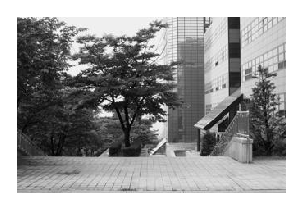
\includegraphics[width=0.23\textwidth]{paper-fig/fig70-1}}\hfill
  \subfigure[ ]{
\includegraphics[width=0.23\textwidth]{paper-fig/fig70-2}}\hfill
  \caption{Expected Likelihood Descriptor}
\end{figure}
\begin{math} L(x) \end{math} can have negative values in static background regions due to the negative log-scaling in (\ref{eq:100}). As next matching stage requires only positive values for computation, the normalization should be performed as,
\begin{equation}\label{eq:140}
  L(x) = 1 - Z \cdot \tilde{L}(x)
\end{equation}
\begin{equation}\label{eq:150}
  Z = \frac{1}{ \sum_x E( \tilde{L}(\hat{x}) ) } \times W \times H \times 0.5
\end{equation}

The \begin{math} W \end{math} and \begin{math} H \end{math} are width and height of the image, respectively. The normalization constant \begin{math} Z \end{math} in (\ref{eq:150}) can be computed by taking sum to one and scaling to uniform distribution with 0.5. After normalizing \begin{math} E(\tilde{L}) \end{math} using (\ref{eq:140}), E-L descriptor ensures that \begin{math} 0 \le E( L(\hat{x})) \le 1 \end{math}. Also, other \begin{math} \tilde{L}( x_i ) \end{math}  can be normalized using \begin{math} Z \end{math}. This normalization transforms unnormalized \begin{math} \tilde{L}( x_i ) \end{math} to be approximately probability values; \begin{math} 0 \le \tilde{L}( x_i ) \approx 1 \end{math}. Some values would exceed \begin{math} 1 \end{math}, but they are unimportant to proceed to the next stage.

The background variation subtraction can be performed by comparing spatial similarity between \begin{math} L(x) \end{math}  and \begin{math} E(\tilde{L}) \end{math}. This is equivalent to shape matching process. Thus, the process can be performed by building local descriptors and then comparing those two descriptors using \begin{math} \chi ^2 \end{math} test (\ref{eq:70}).

A local descriptor for each pixel can be built by sampling local distribution of the \begin{math} L(x) \end{math} into a local histogram. Local smoothness assumption for robustness and centered-focus for distinctiveness can be achieved by building Shape descriptor, \cite{Mikolajczyk, Belongie}. This can be done by center-biased sampling. Figure \ref{fig:80} shows an example. Each box represents a pixel on image patch. The number in each box means an index of the descriptor. The same indexed pixels are taken into a mean for the centered-focus when sampling them into their descriptor. So, 5\begin{math} \times \end{math} 5 spatial distribution can be captured in the 9-bin descriptor. 

\begin{figure}[!t]
  \centering
  \label{fig:80}
  \subfigure[ ]{
\includegraphics[width=0.23\textwidth]{paper-fig/fig80-1}}\hfill
  \subfigure[ ]{
\includegraphics[width=0.23\textwidth]{paper-fig/fig80-2}}
  \caption{Shape Descriptor}
\end{figure}

The foreground likelihood descriptor \begin{math} h_L(x) \end{math} and the expected likelihood descriptor \begin{math} h_b(\hat{x}) \end{math} can be built from \begin{math} L(x), E(L(\hat{x})) \end{math} respectively. The similarity of \begin{math} h_L(x) \end{math}  and \begin{math} h_b(\hat{x}) \end{math} can be obtained using \begin{math} \chi ^2 \end{math} test (\ref{eq:70}) and is called the second-order foreground likelihood \begin{math} L^2(x) \end{math}. Also, the positional displacement within one pixel neighbors is considered using (\ref{eq:120}).

\ref{fig:90} shows an example of variation subtraction process. (a), (b) represent \begin{math} E(\hat{L}) \end{math}. (d), (g) indicates \begin{math} L \end{math}. (e), (h) are \begin{math} L^2 \end{math}. By matching histograms between \begin{math} E(\hat{L}) \end{math} and \begin{math} L, L^2 \end{math} can be obtained. Note that normal dynamic backgrounds are successfully suppressed close to 0, while keeping foregrounds' likelihood from being smoothed.

\begin{figure}[!t]
  \centering
  \label{fig:90}
  \subfigure[ ]{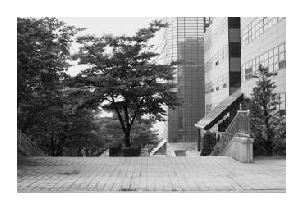
\includegraphics[width=0.23\textwidth]{paper-fig/fig90-a}}\hfill
  \subfigure[ ]{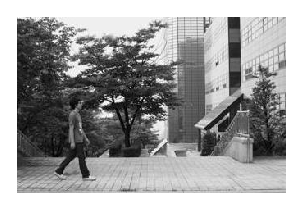
\includegraphics[width=0.23\textwidth]{paper-fig/fig90-b}}\hfill
  \subfigure[ ]{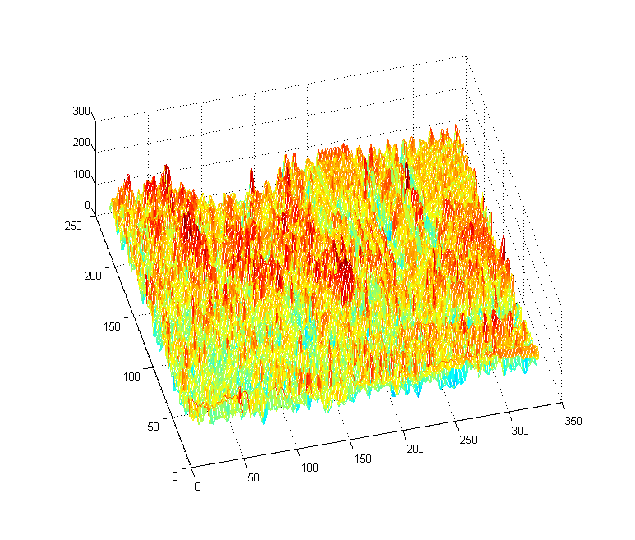
\includegraphics[width=0.15\textwidth]{paper-fig/fig90-c}}\hfill
  \subfigure[ ]{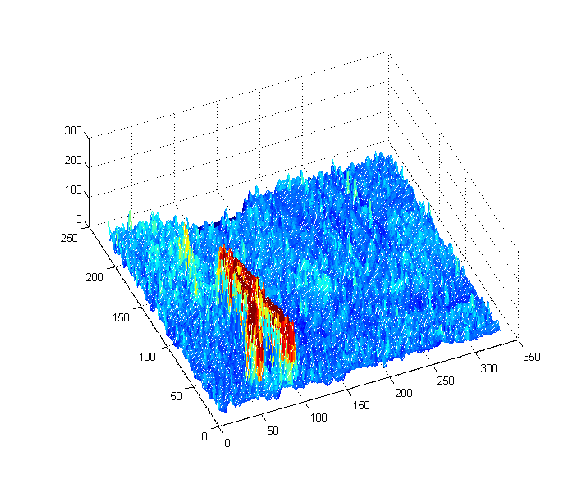
\includegraphics[width=0.15\textwidth]{paper-fig/fig90-d}}\hfill
  \subfigure[ ]{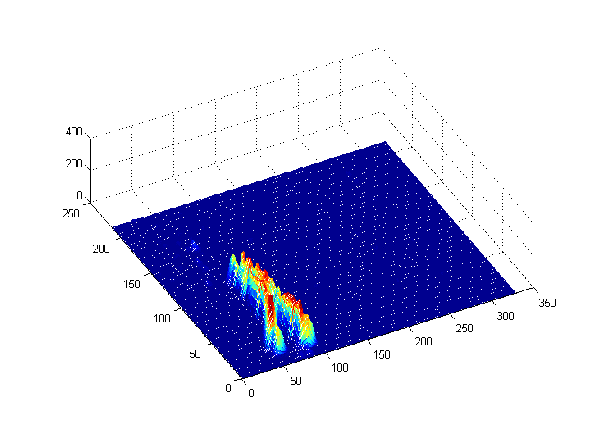
\includegraphics[width=0.15\textwidth]{paper-fig/fig90-e}}\hfill
  \subfigure[ ]{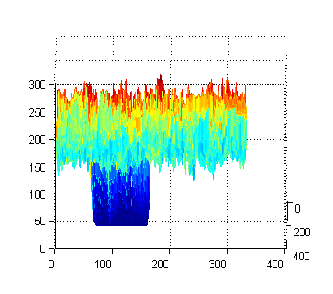
\includegraphics[width=0.15\textwidth]{paper-fig/fig90-f}}\hfill
  \subfigure[ ]{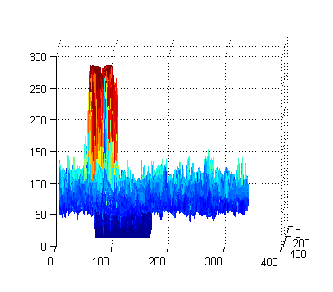
\includegraphics[width=0.15\textwidth]{paper-fig/fig90-g}}\hfill
  \subfigure[ ]{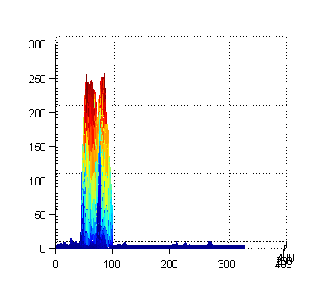
\includegraphics[width=0.15\textwidth]{paper-fig/fig90-h}}
  \caption{Background Variation Subtraction Result}
\end{figure}

\section{Experimental Result}
The algorithm was tested on Natural scenes with dynamic background for object recognition and SEM images with noise for defect detection. Three background models are compared: the temporal model from Elgammal \cite{Elgammal}, the first-order spatio-temporal model, and the second-order spatio-temporal model are illustrated at each column, respectively. In the first row, a positive training example \begin{math} \hat{I}^+ \end{math}, an inspection image \begin{math} I \end{math}, and an expected foreground likelihood \begin{math} E(\hat{L}) \end{math} are shown, respectively.

For balanced comparison, those three models used LRT test for 3 \begin{math} \times \end{math} 3 component  \begin{math} x^C \end{math} (\ref{eq:130}), and considered positional displacement within one pixel (\ref{eq:150}), and used Otsu's thresholding (\ref{eq:100}). Our method was implemented using Matlab and run on 2.40GHz Intel Pentium Core2 Quad processor with 4 GB RAM.

\subsection{Application to Object Recognition of Dynamic scenes}
These image set contain dynamic background, and there are small transitional, rotational misalignments due to camera jitters. Figure \ref{fig:100}–\ref{fig:110} show the results. 

Camouflage problem occurs in the temporal model shown in the first column. The foregrounds having similar intensity to their background were missed. The discrimination is enhanced in the first-order spatio-temporal model in the second column, whereas false-alarms increased. After variation subtraction in the third column, the dynamic backgrounds are successfully suppressed. Also, thanks to the stable response of \begin{math} L^2(x) \end{math} , the global threshold \begin{math} T \end{math} chosen from Otsu's method was working well. Those results show our method is distinctive and robust in dynamic background constraints.

\begin{figure}[!t]
  \centering
  \label{fig:100}
  \subfigure[ ]{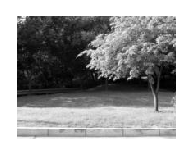
\includegraphics[width=0.15\textwidth]{paper-fig/fig100-1}}\hfill
  \subfigure[ ]{
\includegraphics[width=0.15\textwidth]{paper-fig/fig100-2}}\hfill
  \subfigure[ ]{
\includegraphics[width=0.15\textwidth]{paper-fig/fig100-3}}\hfill
  \subfigure[ ]{
\includegraphics[width=0.15\textwidth]{paper-fig/fig100-4}}\hfill
  \subfigure[ ]{
\includegraphics[width=0.15\textwidth]{paper-fig/fig100-5}}\hfill
  \subfigure[ ]{
\includegraphics[width=0.15\textwidth]{paper-fig/fig100-6}}\hfill
  \subfigure[ ]{
\includegraphics[width=0.15\textwidth]{paper-fig/fig100-7}}\hfill
  \subfigure[ ]{
\includegraphics[width=0.15\textwidth]{paper-fig/fig100-8}}\hfill
  \subfigure[ ]{
\includegraphics[width=0.15\textwidth]{paper-fig/fig100-9}}\hfill
  \subfigure[ ]{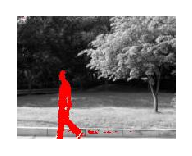
\includegraphics[width=0.15\textwidth]{paper-fig/fig100-10}}\hfill
  \subfigure[ ]{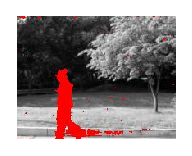
\includegraphics[width=0.15\textwidth]{paper-fig/fig100-11}}\hfill
  \subfigure[ ]{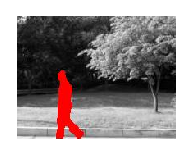
\includegraphics[width=0.15\textwidth]{paper-fig/fig100-12}}
  \caption{Object Recognition on natural scenes. The second row shows foreground likelihoods. The third row shows thresholding images. Those are 194×150 sized images. 32 positive images were used for training. 3 negative images were used for training threshold}
\end{figure}

\begin{figure}[!t]
  \centering
  \label{fig:110}
  \subfigure[ ]{
\includegraphics[width=0.15\textwidth]{paper-fig/fig110-1}}\hfill
  \subfigure[ ]{
\includegraphics[width=0.15\textwidth]{paper-fig/fig110-2}}\hfill
  \subfigure[ ]{
\includegraphics[width=0.15\textwidth]{paper-fig/fig110-3}}\hfill
  \subfigure[ ]{
\includegraphics[width=0.15\textwidth]{paper-fig/fig110-4}}\hfill
  \subfigure[ ]{
\includegraphics[width=0.15\textwidth]{paper-fig/fig110-5}}\hfill
  \subfigure[ ]{
\includegraphics[width=0.15\textwidth]{paper-fig/fig110-6}}\hfill
  \subfigure[ ]{
\includegraphics[width=0.15\textwidth]{paper-fig/fig110-7}}\hfill
  \subfigure[ ]{
\includegraphics[width=0.15\textwidth]{paper-fig/fig110-8}}\hfill
  \subfigure[ ]{
\includegraphics[width=0.15\textwidth]{paper-fig/fig110-9}}\hfill
  \subfigure[ ]{
\includegraphics[width=0.15\textwidth]{paper-fig/fig110-10}}\hfill
  \subfigure[ ]{
\includegraphics[width=0.15\textwidth]{paper-fig/fig110-11}}\hfill
  \subfigure[ ]{
\includegraphics[width=0.15\textwidth]{paper-fig/fig110-12}}
  \caption{Object Recognition on natural scenes. The second row shows foreground likelihoods. The third row shows thresholding images. There are a moving car and walking people behind the tree. Those are 191×148 sized images. 50 positive images were used for training. 3 negative images were used for training threshold}
\end{figure}

\subsection{Application to Defect Detection of Highly Noised SEM images}
These image set contains dynamic textures, and small transitional misalignments. In addition, those are highly noised. Figure \ref{fig:120}–\ref{fig:130} show the results. 

In figure \ref{fig:120}, T-model missed defects having similar colors, which shows it is dull to shape change. The first-order S-T model detected not only shape change, but also more false-alarms, which means it is vulnerable to noise. However, the false-positives are suppressed in the second-order S-T model. In figure \ref{fig:130}, due to the significant noise, T-model and first order S-T model failed to correct localizing defects, whereas our second-order S-T model successfully suppressed noises and detected correctly.

A decision of defect image is crucial in defect detection. Thus, the classification rate has been used for performance evaluation. Table \ref{tab:10} shows the classification rate of the defect detection in SEM images. Note that false positives are significantly decreased.

\begin{table}[!t]
  \centering
  \label{tab:10}
  \caption{Classification rate for defect detection}
\end{table}

\begin{figure}[t]
  \centering
  \label{fig:120}
  \subfigure[ ]{
\includegraphics[width=0.15\textwidth]{paper-fig/fig120-1}}\hfill
  \subfigure[ ]{
\includegraphics[width=0.15\textwidth]{paper-fig/fig120-2}}\hfill
  \subfigure[ ]{\includegraphics[width=0.15\textwidth]{paper-fig/fig120-3}}\hfill
  \subfigure[ ]{\includegraphics[width=0.15\textwidth]{paper-fig/fig120-4}}\hfill
  \subfigure[ ]{\includegraphics[width=0.15\textwidth]{paper-fig/fig120-5}}\hfill
  \subfigure[ ]{\includegraphics[width=0.15\textwidth]{paper-fig/fig120-6}}\hfill
  \subfigure[ ]{\includegraphics[width=0.15\textwidth]{paper-fig/fig120-7}}\hfill
  \subfigure[ ]{\includegraphics[width=0.15\textwidth]{paper-fig/fig120-8}}\hfill
  \subfigure[ ]{\includegraphics[width=0.15\textwidth]{paper-fig/fig120-9}}\hfill
  \subfigure[ ]{\includegraphics[width=0.15\textwidth]{paper-fig/fig120-10}}\hfill
  \subfigure[ ]{\includegraphics[width=0.15\textwidth]{paper-fig/fig120-11}}\hfill
  \subfigure[ ]{\includegraphics[width=0.15\textwidth]{paper-fig/fig120-12}}
  \caption{Defect Detection on SEM images. The second row shows foreground likelihoods. The third row shows thresholding images. Those are 111×111 sized images. 33 positive images were used for training. 3 negative images were used for training threshold.}
\end{figure}

\begin{figure}[!t]
  \centering
  \label{fig:130}
  \subfigure[ ]{\includegraphics[width=0.15\textwidth]{paper-fig/fig130-1}}\hfill
  \subfigure[ ]{\includegraphics[width=0.15\textwidth]{paper-fig/fig130-2}}\hfill
  \subfigure[ ]{\includegraphics[width=0.15\textwidth]{paper-fig/fig130-3}}\hfill
  \subfigure[ ]{\includegraphics[width=0.15\textwidth]{paper-fig/fig130-4}}\hfill
  \subfigure[ ]{\includegraphics[width=0.15\textwidth]{paper-fig/fig130-5}}\hfill
  \subfigure[ ]{\includegraphics[width=0.15\textwidth]{paper-fig/fig130-6}}\hfill
  \subfigure[ ]{\includegraphics[width=0.15\textwidth]{paper-fig/fig130-7}}\hfill
  \subfigure[ ]{\includegraphics[width=0.15\textwidth]{paper-fig/fig130-8}}\hfill
  \subfigure[ ]{\includegraphics[width=0.15\textwidth]{paper-fig/fig130-9}}\hfill
  \subfigure[ ]{\includegraphics[width=0.15\textwidth]{paper-fig/fig130-10}}\hfill
  \subfigure[ ]{\includegraphics[width=0.15\textwidth]{paper-fig/fig130-11}}\hfill
  \subfigure[ ]{\includegraphics[width=0.15\textwidth]{paper-fig/fig130-12}}
  \caption{Defect Detection on SEM images. The second row shows foreground likelihoods. The third row shows thresholding images. Those are 110×109 sized images. 22 positive images were used for training. 3 negative images were used for training threshold.}
\end{figure}



\section{Conclusion}

The dynamic background constraints demand distinctiveness and robustness of the background model: camouflage problem and dynamic background problem. Therefore, we extended the background model by assuming S-T MRF for overcoming those problems: the spatio-temporal consistency in the first-order space for distinctiveness and variation consistency in the second-order space for robustness. We showed the distinctiveness and robustness in the applications of the object recognition of dynamic scenes and defect detection in highly noised SEM images.
The suggested model can be easily applied to video case by updating expected likelihood descriptor \begin{math} h_B(\hat{x}) \end{math} as,
\begin{equation}\label{eq:160}
  h_B(\hat{x}) = (1 - \alpha) \cdot h_B(\hat{x}) + \alpha \cdot h_L(x)
\end{equation}

where α is a learning rate. 
The suggested method has the same limitation as other background subtraction methods. Kernel density estimation requires considerable computation for inspection as it is a kind of instance based learning. The main reason of the use of the instance based learning results from the high dimensionality of the feature space for description of the background density. However, defect detection on SEM images and object recognition on video requires real-time solution for detection, so eager learning is more desirable. Also, a study of illumination or rotation change is needed for more robustness of the background model.

\section*{Acknowledgement}






% \bibliographystyle{IEEEtran}
% \bibliograph{IEEEabrv,yw_paper1}



%\bibliographystyle{ams[lain}
%\bibliography{test}

\begin{thebibliography}{19}

\bibitem{Kamijo}
  S. Kamijo, K. Ikeuchi, and M. Sakauchi. Segmentations of spatio- temporal images by spatio-temporal Markov random field model. Proc. EMMCVPR Workshop, pp. 298-313, 2001.

\bibitem{Piccardi}
  M. Piccardi. Background subtraction techniques: a review. In Proc. IEEE Int. Conf. Systems, Man, Cybernetics, pp. 3099–3104, 2004.

\bibitem{Wren}
  C. Wren, A. Azarbayejani, T. Darrel, and A. Pentland. Pfinder: Real time tracking of the human body. In IEEE Transactions on Pattern Analysis and Machine Intelligence, 1997.

\bibitem{Cucchiara}
  R. Cucchiara, C. Grana, M. Piccardi, and A. Prati. Detecting moving objects, ghosts, and shadows in video streams. IEEE Trans. on Pattern Anal. and Machine Intell., vol. 25, no. 10, pp. 1337-1442, 2003.

\bibitem{Stauffer}
  C. Stauffer and W.E.L. Grimson. Adaptive background mixture models for real-time tracking. Proc. IEEE CVPR, pp. 246-252, 1999.

\bibitem{Elgammal}
  A. Elgammal, D. Harwood, and L. Davis. Non-parametric Model for Background Subtraction. Proc. European Conf. Computer Vision, vol. 2, pp. 751-767, June 2000.

\bibitem{Sheikh}
  Y. Sheikh, M. Shah. Bayesian modelling of dynamic scenes for object detection. IEEE Transactions on Pattern Analysis and Machine Intelligence. 27 (11) pp. 1778–1792, 2005.

\bibitem{Ko}
  T. Ko, S. Soatto, and D. Estrin. Background subtraction on distributions. In ECCV, volume 3, pp 276–289, 2008.

\bibitem{Mittal}
  A. Mittal, and N. Paragios. Motion-based background subtraction using adaptive kernel density estimation. In IEEE Proceedings on Computer Vision and Pattern Recognition, 2004.

\bibitem{Jodoin}
  P.-M. Jodoin, J.Konrad, and V. Saligrama. Modeling background activity for behavior subtraction. In proc. of IEEE ICDSC, 2008.

\bibitem{Bebezeth}
  Y. Bebezeth, P.-M. Jodoin, V. Saligrama, C. Rosenberger, Abnormal events detection based on spatio-temporal co-occurences. In IEEE Proceedings on Computer Vision and Pattern Recognition, pp. 2458–2465, 2009.

\bibitem{Mikolajczyk}
  K. Mikolajczyk, and C. Schmid. A performance evaluation of local descriptors. In Proceedings of the Conference on Computer Vision and Pattern Recognition, pp. 257–264, 2003.

\bibitem{Lowe}
  D. Lowe. Distinctive image features from scale-invariant keypoints. International Journal of Computer Vision, 2(60):91.110, 2004.

\bibitem{Belongie}
  S. Belongie, J. Malik, and J. Puzicha. Shape matching and object recognition using shape contexts. IEEE Transactions on Pattern Analysis and Machine Intelligence, 24(4):509.522, 2002.

\bibitem{Sezgin}
  M. Sezgin, B. Sankur. Survey over image thresholding techniques and quantitative performance evaluation. Journal of Electronic Imaging, vol. 13, no. 1, pp. 146–165, 2004.

\bibitem{Otsu}
  N. Otsu. A threshold selection method from gray level histograms. IEEE Trans. Syst. Man Cybern. SMC-9, pp. 62–66, 1979.

\bibitem{Bishop}
  C. M. Bishop. Pattern Recognition and Machine Learning. Springer, August 2006.

\bibitem{Jones}
  M. C. Jones, J. S. Marron, and S. J. Sheather. A Brief Survey of Bandwidth Selection for Density Estimation. Journal of the American Statistical Association, Vol. 91, No. 433, 401-407, 1996.

\bibitem{Comaniciu}
  D. Comaniciu, V. Ramesh, and P. Meer. The Variable Bandwidth Mean Shift and Data-Driven Scale Selection. Proc Eighth International Conference of Computer Vision, vol. I, pp. 438-445, 2001

\end{thebibliography}



\end{document}


